% Options for packages loaded elsewhere
\PassOptionsToPackage{unicode}{hyperref}
\PassOptionsToPackage{hyphens}{url}
\PassOptionsToPackage{dvipsnames,svgnames,x11names}{xcolor}
%
\documentclass[
  letterpaper,
  DIV=11,
  numbers=noendperiod]{scrreprt}

\usepackage{amsmath,amssymb}
\usepackage{lmodern}
\usepackage{iftex}
\ifPDFTeX
  \usepackage[T1]{fontenc}
  \usepackage[utf8]{inputenc}
  \usepackage{textcomp} % provide euro and other symbols
\else % if luatex or xetex
  \usepackage{unicode-math}
  \defaultfontfeatures{Scale=MatchLowercase}
  \defaultfontfeatures[\rmfamily]{Ligatures=TeX,Scale=1}
\fi
% Use upquote if available, for straight quotes in verbatim environments
\IfFileExists{upquote.sty}{\usepackage{upquote}}{}
\IfFileExists{microtype.sty}{% use microtype if available
  \usepackage[]{microtype}
  \UseMicrotypeSet[protrusion]{basicmath} % disable protrusion for tt fonts
}{}
\makeatletter
\@ifundefined{KOMAClassName}{% if non-KOMA class
  \IfFileExists{parskip.sty}{%
    \usepackage{parskip}
  }{% else
    \setlength{\parindent}{0pt}
    \setlength{\parskip}{6pt plus 2pt minus 1pt}}
}{% if KOMA class
  \KOMAoptions{parskip=half}}
\makeatother
\usepackage{xcolor}
\setlength{\emergencystretch}{3em} % prevent overfull lines
\setcounter{secnumdepth}{1}
% Make \paragraph and \subparagraph free-standing
\ifx\paragraph\undefined\else
  \let\oldparagraph\paragraph
  \renewcommand{\paragraph}[1]{\oldparagraph{#1}\mbox{}}
\fi
\ifx\subparagraph\undefined\else
  \let\oldsubparagraph\subparagraph
  \renewcommand{\subparagraph}[1]{\oldsubparagraph{#1}\mbox{}}
\fi


\providecommand{\tightlist}{%
  \setlength{\itemsep}{0pt}\setlength{\parskip}{0pt}}\usepackage{longtable,booktabs,array}
\usepackage{calc} % for calculating minipage widths
% Correct order of tables after \paragraph or \subparagraph
\usepackage{etoolbox}
\makeatletter
\patchcmd\longtable{\par}{\if@noskipsec\mbox{}\fi\par}{}{}
\makeatother
% Allow footnotes in longtable head/foot
\IfFileExists{footnotehyper.sty}{\usepackage{footnotehyper}}{\usepackage{footnote}}
\makesavenoteenv{longtable}
\usepackage{graphicx}
\makeatletter
\def\maxwidth{\ifdim\Gin@nat@width>\linewidth\linewidth\else\Gin@nat@width\fi}
\def\maxheight{\ifdim\Gin@nat@height>\textheight\textheight\else\Gin@nat@height\fi}
\makeatother
% Scale images if necessary, so that they will not overflow the page
% margins by default, and it is still possible to overwrite the defaults
% using explicit options in \includegraphics[width, height, ...]{}
\setkeys{Gin}{width=\maxwidth,height=\maxheight,keepaspectratio}
% Set default figure placement to htbp
\makeatletter
\def\fps@figure{htbp}
\makeatother
\newlength{\cslhangindent}
\setlength{\cslhangindent}{1.5em}
\newlength{\csllabelwidth}
\setlength{\csllabelwidth}{3em}
\newlength{\cslentryspacingunit} % times entry-spacing
\setlength{\cslentryspacingunit}{\parskip}
\newenvironment{CSLReferences}[2] % #1 hanging-ident, #2 entry spacing
 {% don't indent paragraphs
  \setlength{\parindent}{0pt}
  % turn on hanging indent if param 1 is 1
  \ifodd #1
  \let\oldpar\par
  \def\par{\hangindent=\cslhangindent\oldpar}
  \fi
  % set entry spacing
  \setlength{\parskip}{#2\cslentryspacingunit}
 }%
 {}
\usepackage{calc}
\newcommand{\CSLBlock}[1]{#1\hfill\break}
\newcommand{\CSLLeftMargin}[1]{\parbox[t]{\csllabelwidth}{#1}}
\newcommand{\CSLRightInline}[1]{\parbox[t]{\linewidth - \csllabelwidth}{#1}\break}
\newcommand{\CSLIndent}[1]{\hspace{\cslhangindent}#1}

\newenvironment{cols}[1][]{}{}

\newenvironment{col}[1]{
\begin{minipage}{#1}\ignorespaces}{%
\end{minipage}
\ifhmode\unskip\fi
\aftergroup\useignorespacesandallpars}

\def\useignorespacesandallpars#1\ignorespaces\fi{%
#1\fi\ignorespacesandallpars}

\makeatletter
\def\ignorespacesandallpars{%
  \@ifnextchar\par
    {\expandafter\ignorespacesandallpars\@gobble}%
    {}%
}
\makeatother
\usepackage{booktabs}
\usepackage{caption}
\usepackage{longtable}
\KOMAoption{captions}{tableheading}
\makeatletter
\makeatother
\makeatletter
\@ifpackageloaded{bookmark}{}{\usepackage{bookmark}}
\makeatother
\makeatletter
\@ifpackageloaded{caption}{}{\usepackage{caption}}
\AtBeginDocument{%
\ifdefined\contentsname
  \renewcommand*\contentsname{Table of contents}
\else
  \newcommand\contentsname{Table of contents}
\fi
\ifdefined\listfigurename
  \renewcommand*\listfigurename{List of Figures}
\else
  \newcommand\listfigurename{List of Figures}
\fi
\ifdefined\listtablename
  \renewcommand*\listtablename{List of Tables}
\else
  \newcommand\listtablename{List of Tables}
\fi
\ifdefined\figurename
  \renewcommand*\figurename{Figure}
\else
  \newcommand\figurename{Figure}
\fi
\ifdefined\tablename
  \renewcommand*\tablename{Table}
\else
  \newcommand\tablename{Table}
\fi
}
\@ifpackageloaded{float}{}{\usepackage{float}}
\floatstyle{ruled}
\@ifundefined{c@chapter}{\newfloat{codelisting}{h}{lop}}{\newfloat{codelisting}{h}{lop}[chapter]}
\floatname{codelisting}{Listing}
\newcommand*\listoflistings{\listof{codelisting}{List of Listings}}
\makeatother
\makeatletter
\@ifpackageloaded{caption}{}{\usepackage{caption}}
\@ifpackageloaded{subcaption}{}{\usepackage{subcaption}}
\makeatother
\makeatletter
\@ifpackageloaded{tcolorbox}{}{\usepackage[many]{tcolorbox}}
\makeatother
\makeatletter
\@ifundefined{shadecolor}{\definecolor{shadecolor}{rgb}{.97, .97, .97}}
\makeatother
\makeatletter
\makeatother
\ifLuaTeX
  \usepackage{selnolig}  % disable illegal ligatures
\fi
\IfFileExists{bookmark.sty}{\usepackage{bookmark}}{\usepackage{hyperref}}
\IfFileExists{xurl.sty}{\usepackage{xurl}}{} % add URL line breaks if available
\urlstyle{same} % disable monospaced font for URLs
\hypersetup{
  pdftitle={Introduction to Statistics and Data Science: Instructor's Guide},
  pdfauthor={Danielle Sass},
  colorlinks=true,
  linkcolor={blue},
  filecolor={Maroon},
  citecolor={Blue},
  urlcolor={Blue},
  pdfcreator={LaTeX via pandoc}}

\title{Introduction to Statistics and Data Science: Instructor's Guide}
\author{Danielle Sass}
\date{2023-10-04}

\begin{document}
\maketitle
\ifdefined\Shaded\renewenvironment{Shaded}{\begin{tcolorbox}[breakable, interior hidden, enhanced, boxrule=0pt, sharp corners, borderline west={3pt}{0pt}{shadecolor}, frame hidden]}{\end{tcolorbox}}\fi

\renewcommand*\contentsname{Table of contents}
{
\hypersetup{linkcolor=}
\setcounter{tocdepth}{1}
\tableofcontents
}
\bookmarksetup{startatroot}

\hypertarget{preface}{%
\chapter*{Preface}\label{preface}}
\addcontentsline{toc}{chapter}{Preface}

This book is meant to be a resource for instructors to provide a
complete guide for teaching Introduction to Statistics and Data Science.

All activities and lecture slides can be downloaded from the Posit Cloud
\href{https://posit.cloud/content/6672899}{ISDS Course Content}

Reading Tutorials are completed using RStudio. Visit the
\href{https://nustat.github.io/isdsTutorials/}{isdsTutorials website}
for information on how to install the package and run the tutorials.

\begin{cols}

\begin{col}{0.1\textwidth}
\includegraphics[width=1.12em,height=1em]{./index_files/figure-pdf/fa-icon-a26fb0a0e540e124bcdee28d951f0027.pdf}

\end{col}

\begin{col}{0.85\textwidth}
This icon indicates a tip/suggestion!

\end{col}

\end{cols}

\includegraphics[width=1.12em,height=1em]{./index_files/figure-pdf/fa-icon-a26fb0a0e540e124bcdee28d951f0027.pdf}

This icon indicates a tip/suggestion!

\includegraphics[width=1.12em,height=1em]{./index_files/figure-pdf/fa-icon-a26fb0a0e540e124bcdee28d951f0027.pdf}
This icon indicates a tip/suggestion!

\bookmarksetup{startatroot}

\hypertarget{sample-syllabus}{%
\chapter*{Sample syllabus}\label{sample-syllabus}}
\addcontentsline{toc}{chapter}{Sample syllabus}

\hypertarget{course-info}{%
\section*{Course info}\label{course-info}}
\addcontentsline{toc}{section}{Course info}

\begin{longtable}[]{@{}llll@{}}
\toprule()
& Day & Time & Location \\
\midrule()
\endhead
Lectures & MWF & 9:00 am - 9:50 am & Room 107 \\
\bottomrule()
\end{longtable}

\textbf{Prerequisite:} High School Algebra

\hypertarget{instructional-team}{%
\section*{Instructional Team}\label{instructional-team}}
\addcontentsline{toc}{section}{Instructional Team}

\begin{longtable}[]{@{}llll@{}}
\toprule()
& Title & Email & Office Hours \\
\midrule()
\endhead
Prof.~Name & Professor & & By Appointment \\
TA Name & TA & & Tue/Thur 4-5pm \\
\bottomrule()
\end{longtable}

\hypertarget{learning-objectives}{%
\section*{Learning objectives}\label{learning-objectives}}
\addcontentsline{toc}{section}{Learning objectives}

By the end of the quarter, you will be able to\ldots{}

\begin{enumerate}
\def\labelenumi{\arabic{enumi}.}
\tightlist
\item
  Use statistical software to manage and process data.
\item
  Use statistical software to perform exploratory data analyses. That
  is, explore data numerically and visually to gain understanding
  through data and generate hypotheses and inferences to later test.
\end{enumerate}

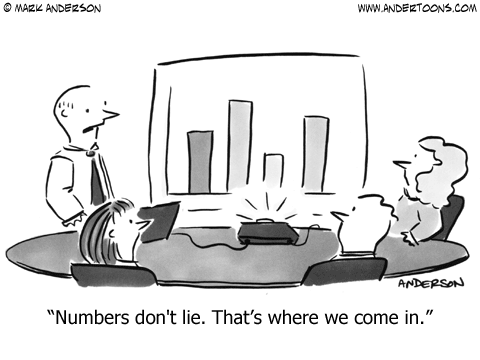
\includegraphics[width=0.5\textwidth,height=\textheight]{./images/cartoon3308.png}

\begin{enumerate}
\def\labelenumi{\arabic{enumi}.}
\setcounter{enumi}{2}
\tightlist
\item
  Recognize the importance of data collection, identify limitations in
  data collection methods, and determine how they affect the scope of
  inference.
\item
  Build a conceptual understanding of the unified nature of statistical
  inference.
\item
  Apply estimation and testing methods to analyze single variables or
  the relationship between two variables in order to understand natural
  phenomena and make data-based decisions.
\item
  Model numerical response variables using a single or multiple
  explanatory variables.
\item
  Interpret results in context without relying on statistical jargon.
\item
  Critique and evaluate data-based claims and decisions.
\end{enumerate}

\hypertarget{course-structure}{%
\section*{Course Structure}\label{course-structure}}
\addcontentsline{toc}{section}{Course Structure}

This class will follow an active learning design. Meaning the majority
of each lecture will be dedicated to working on activities. A lot of
what you do in this course will involve writing code, and coding is a
skill that is best learned by doing. A typical class will devote 10-15
minutes to discussion/lecture with the remainder of the class devoted to
working on activities where students will either work by themselves or
in groups. Throughout the class we will discuss and review the work on
the activities. In many cases we may come together to work on parts of
an activity as a class.

\hypertarget{textbooks}{%
\section*{Textbooks}\label{textbooks}}
\addcontentsline{toc}{section}{Textbooks}

We will be using
\href{https://nustat.github.io/intro-stat-data-sci/}{Introduction to
Statistics and Data Science} which is a free online book that we have
been developing for this course.

\hypertarget{software}{%
\section*{Software}\label{software}}
\addcontentsline{toc}{section}{Software}

We will be using/introducing the free statistical software
\href{https://posit.cloud/}{Posit Cloud}.

\hypertarget{hardware}{%
\section*{Hardware}\label{hardware}}
\addcontentsline{toc}{section}{Hardware}

Students will need a laptop or Chromebook to be able to follow lectures
and to work with RStudio Cloud to complete activities. If access to a
laptop is an issue, then please contact the course instructor and we
will work to find an accommodation.

\hypertarget{assessment}{%
\section*{Assessment}\label{assessment}}
\addcontentsline{toc}{section}{Assessment}

Assessment for the course is comprised of five components:
participation, reading tutorials, activities, 3 exams, and final
project.

\hypertarget{participation}{%
\subsection*{Participation}\label{participation}}
\addcontentsline{toc}{subsection}{Participation}

\hypertarget{reading-tutorials}{%
\subsection*{Reading Tutorials}\label{reading-tutorials}}
\addcontentsline{toc}{subsection}{Reading Tutorials}

Reading tutorials will be completed using Posit Cloud/Rstudio and
uploaded to the course Canvas page. Each reading tutorial will be scaled
to be worth 10 points. Reading tutorials will be accepted up to 3 days
after the due date with a 10\% late penalty.

\emph{The lowest reading tutorial grade will be dropped at the end of
the semester.}

\hypertarget{activities}{%
\subsection*{Activities}\label{activities}}
\addcontentsline{toc}{subsection}{Activities}

Daily activities will be worth 10 points. Activities will be accepted up
to 3 days after the due date with a 10\% late penalty.

\emph{The lowest activity grade will be dropped at the end of the
semester.}

\hypertarget{exams}{%
\subsection*{Exams}\label{exams}}
\addcontentsline{toc}{subsection}{Exams}

There will be 3 in-class exams; they will be structured very similarly
to your reading tutorials. Roughly half of it will focus on conceptual
knowledge and roughly half will focus on practical applications.
Students will be allowed one 8.5 x 11 inch cheat sheet (front \& back)
on each in-class exams. The exams are not cumulative.

\hypertarget{project}{%
\subsection*{Project}\label{project}}
\addcontentsline{toc}{subsection}{Project}

The final project will be completed in groups of 3-6 people and allow
you to explore a dataset of your choice. More information will be
provided later in the quarter.

\hypertarget{exam-improvement-policy}{%
\subsection*{Exam Improvement Policy}\label{exam-improvement-policy}}
\addcontentsline{toc}{subsection}{Exam Improvement Policy}

We have worked to develop a policy geared towards a growth mindset. That
is, we want a policy where students clearly demonstrate that they have
used the exam as a diagnostic tool to learn from and improve their
understanding of statistics. There is NO final cumulative exam during
the designated final exam time, instead you may choose to retake 1 exam
during the exam time. This exam will replace your old score --- only in
cases where it is an improvement.

\hypertarget{missed-exam-policy}{%
\subsection*{Missed Exam Policy}\label{missed-exam-policy}}
\addcontentsline{toc}{subsection}{Missed Exam Policy}

There are no make-up exams. If you miss an exam due to illness, travel,
etc., you will need to take the exam during the final exam period as
your re-take exam.

\hypertarget{grading}{%
\section*{Grading}\label{grading}}
\addcontentsline{toc}{section}{Grading}

The final course grade will be calculated as follows:

\begin{longtable}[]{@{}ll@{}}
\toprule()
Category & Percentage \\
\midrule()
\endhead
Participation & 5\% \\
Reading Tutorials & 15\% \\
Activities & 10\% \\
Exam 1 & 20\% \\
Exam 2 & 20\% \\
Exam 3 & 20\% \\
Project & 10\% \\
\bottomrule()
\end{longtable}

The final letter grade will be determined based on the following
thresholds:

\begin{longtable}[]{@{}ll@{}}
\toprule()
Letter Grade & Final Grade \\
\midrule()
\endhead
A & \textgreater= 93 \\
A- & 90 - 92.9 \\
B+ & 87 - 89.9 \\
B & 83 - 86.9 \\
B- & 80 - 82.9 \\
C+ & 77 - 79.9 \\
C & 73 - 76.9 \\
C- & 70 - 72.9 \\
D & 60 - 69.9 \\
F & \textless{} 59.9 \\
\bottomrule()
\end{longtable}

\hypertarget{tips-for-success}{%
\section*{Tips for success}\label{tips-for-success}}
\addcontentsline{toc}{section}{Tips for success}

\begin{itemize}
\tightlist
\item
  Dedicate yourself to being an active and engaged learner.
\item
  Prepare for class by \emph{reading and working} through code
  \emph{before} class.
\item
  Work in groups to learn and complete activities.
\item
  Ask questions! Ask them during class, office hours, or on Campuswire.
\item
  Contribute to a welcoming and inclusive learning environment.
\item
  Don't be afraid to make mistakes, you learn from mistakes.
\end{itemize}

\hypertarget{asking-questions-course-communication}{%
\section*{Asking Questions \& Course
Communication}\label{asking-questions-course-communication}}
\addcontentsline{toc}{section}{Asking Questions \& Course Communication}

This term we will be using \href{https://campuswire.com}{Campuswire}
(``Enrollment Code: XXXX'') as our preferred platform for questions
about activities, reading tutorials, and general course questions. The
system is highly catered to getting you help quickly and efficiently
from classmates and the instructional team. Rather than emailing
questions to the instructional team, you should post your questions on
Campuswire.

The instructional team will check Campuswire periodically and answer
questions, but we strongly encourage students to answer each other's
questions. To this end, student will be able to earn bonus points ---
see Canvas for details.

Please do not expect answers during weekends and evenings.

\hypertarget{school-policies}{%
\section*{School Policies}\label{school-policies}}
\addcontentsline{toc}{section}{School Policies}

Add your standard school policies here.

\bookmarksetup{startatroot}

\hypertarget{tentative-schedule}{%
\chapter*{Tentative schedule}\label{tentative-schedule}}
\addcontentsline{toc}{chapter}{Tentative schedule}

\hypertarget{week-schedule}{%
\section*{11 week Schedule}\label{week-schedule}}
\addcontentsline{toc}{section}{11 week Schedule}

\begin{longtable}[]{@{}
  >{\raggedright\arraybackslash}p{(\columnwidth - 6\tabcolsep) * \real{0.2027}}
  >{\raggedright\arraybackslash}p{(\columnwidth - 6\tabcolsep) * \real{0.3514}}
  >{\raggedright\arraybackslash}p{(\columnwidth - 6\tabcolsep) * \real{0.2432}}
  >{\raggedright\arraybackslash}p{(\columnwidth - 6\tabcolsep) * \real{0.2027}}@{}}
\toprule()
\begin{minipage}[b]{\linewidth}\raggedright
\end{minipage} & \begin{minipage}[b]{\linewidth}\raggedright
Topic
\end{minipage} & \begin{minipage}[b]{\linewidth}\raggedright
Textbook
\end{minipage} & \begin{minipage}[b]{\linewidth}\raggedright
Agenda
\end{minipage} \\
\midrule()
\endhead
Day 1 & Syllabus Day & & Syllabus Day \\
Day 2 & Intro to R & Preface and Chapter 1 & Activity 01 \\
Day 3 & Data Visualization & Sections 2.0-2.3 & Activity 02 \\
Day 4 & Data Visualization & Sections 2.4-2.6 & Activity 03 \\
Day 5 & Data Visualization & Sections 2.7-2.9 & Activity 04 \\
Day 6 & Data Wrangling & Sections 3.0-3.3 & Activity 05 \\
Day 7 & Data Wrangling & Sections 3.4-3.9 & Activity 06 \\
Day 8 & Tidy Data & Chapter 4 & Activity 07 \\
Day 9 & Exam 1 & & \\
Day 10 & Regression & Sections 5.0-5.1 & Activity 08 \\
Day 11 & Regression & Sections 5.2-5.4 & Activity 09 \\
Day 12 & Regression & Sections 6.0-6.1 & Activity 10 \\
Day 13 & Regression & Sections 6.2-6.4 & Activity 11 \\
Day 14 & Randomization + Causality & Chapter 7 & Activity 12 \\
Day 15 & Populations + Generalizability & Chapter 8 & Activity 13 \\
Day 16 & Exam 2 & & \\
Day 17 & Distributions & Sections 9.0-9.1 & Activity 14 \\
Day 18 & Repeated Sampling & Sections 9.2-9.4 & Activity 15 \\
Day 19 & CLT & Sections 9.5-9.7 & Activity 16 \\
Day 20 & Confidence Intervals & Chapter 10 & Activity 17 \\
Day 21 & Confidence Intervals & Chapter 10 & Activity 17 \\
Day 22 & P-values & Chapter 11 & Activity 18 \\
Day 23 & Hypothesis Testing & Chapter 12 & Activity 19 \\
Day 24 & Hypothesis Testing & Chapter 12 & Activity 20 \\
Day 25 & Hypothesis Testing & Chapter 12 & Activity 20 \\
Day 26 & Review & Chapter 13 & \\
Day 27 & Exam 3 & & \\
& Final Project & & \\
\bottomrule()
\end{longtable}

\bookmarksetup{startatroot}

\hypertarget{day-01}{%
\chapter*{Day 01}\label{day-01}}
\addcontentsline{toc}{chapter}{Day 01}

Welcome to class! Today is all about getting setup with the needed
resources and reviewing the syllabus.

\hypertarget{agenda}{%
\section*{Agenda}\label{agenda}}
\addcontentsline{toc}{section}{Agenda}

\begin{longtable}{ll}
\toprule
time & agenda \\ 
\midrule
15 min & Syllabus and expectations \\ 
20 min & Welcome and get students setup with all of the needed resources \\ 
15 min & Students take survey and get to know their neighbors \\ 
\bottomrule
\end{longtable}

\hypertarget{todays-tasks}{%
\section*{Today's tasks}\label{todays-tasks}}
\addcontentsline{toc}{section}{Today's tasks}

\begin{cols}

\begin{col}{0.15\textwidth}
\includegraphics[width=1.12em,height=1em]{./01-content_files/figure-pdf/fa-icon-a26fb0a0e540e124bcdee28d951f0027.pdf}

\end{col}

\begin{col}{0.85\textwidth}
I recommend using Posit Cloud if possible for ease of getting started.
Otherwise you will need to dedicate more time towards downloading R and
RStudio.

See the sample survey for some examples of questions to ask your
students! We use these survey results on the exams.

\end{col}

\end{cols}

Make sure you have completed the following agenda items by the end of
class!

\begin{enumerate}
\def\labelenumi{\arabic{enumi}.}
\tightlist
\item
  Review the syllabus
\item
  Visit the course's \href{https://campuswire.com}{Campuswire page}
  using your school email. Enrollment code: XXXX
\item
  We will be using \href{https://ahaslides.com}{AHA slides} for
  participation.
\item
  Gain access to the Posit Cloud Class Workspace or install R and
  RStudio
\item
  Set up and test out the Reading Tutorials System. Install the required
  package:
  \texttt{remotes::install\_github("NUstat/isdsTutorials",\ dependencies\ =\ TRUE)}
  Try running the first tutorial:
  \texttt{learnr::run\_tutorial("01\_intro",\ package\ =\ "isdsTutorials")}
\item
  Login/create your \href{https://northwestern.zoom.us/}{Northwestern
  Zoom Account} if you do not have one. This will be used for office
  hours or requested appointments.
\item
  Complete the \href{https://forms.gle/eoPS2oXfPumsWaCd7}{google survey}
  - we will use this data later.
\end{enumerate}

\hypertarget{homework}{%
\section*{Homework}\label{homework}}
\addcontentsline{toc}{section}{Homework}

\begin{itemize}
\item
  Read \href{https://nustat.github.io/intro-stat-data-sci/}{Preface and
  Chapter 1} of the book
\item
  Complete RT 01 by running
  \texttt{learnr::run\_tutorial("01\_intro",\ package\ =\ "isdsTutorials")}
  in your Console and submitting the downloaded html to a learning
  management system
\end{itemize}

\bookmarksetup{startatroot}

\hypertarget{references}{%
\chapter*{References}\label{references}}
\addcontentsline{toc}{chapter}{References}

\hypertarget{refs}{}
\begin{CSLReferences}{0}{0}
\end{CSLReferences}



\end{document}
